% Draft 3, 2026-10-16.
% ACL template (acl.sty), preprint mode.
% Source of truth for every number:
%   confirmatory run          -> artifacts/confirmatory/analysis.json, docs/confirmatory-results.md
%   run D                     -> artifacts/retrieval-suppression/analysis.json, docs/retrieval-suppression-results.md
%   Jev re-run                -> artifacts/jev-rerun/analysis.json, docs/jev-rerun-results.md
%   post hoc (round 3)        -> artifacts/posthoc/round3.json, docs/posthoc-round3.md
%   post hoc (round 3 review) -> artifacts/posthoc/round3b.json, docs/posthoc-round3b.md
%   run D2                    -> artifacts/retrieval-mechanism/analysis.json, docs/retrieval-mechanism-results.md
%   exploratory record        -> artifacts/revision/analysis.json
\documentclass[11pt]{article}

% Official ACL style (github.com/acl-org/acl-style-files, commit d5adc823). Use [review] for an anonymous submission.
\usepackage[preprint]{acl}
\usepackage{times}
\usepackage{latexsym}
\usepackage[T1]{fontenc}
\usepackage[utf8]{inputenc}
\usepackage{microtype}
\usepackage{inconsolata}
\usepackage{amsmath}
\usepackage{booktabs}
\usepackage{graphicx}
\usepackage{xcolor}
\usepackage{tikz}
\usetikzlibrary{arrows.meta,positioning,calc}
\usepackage{cleveref}

\graphicspath{{../docs/figures/}}
\setlength{\tabcolsep}{4pt}

\title{Matched data, small gaps: a pre-registered comparison of fine-tuned classifiers, retrieval-prompted language models and a typed-decision model for intent and out-of-scope decisions}
\author{Safwan Kamal}

\begin{document}
\maketitle
\begin{abstract}
We compare a fine-tuned 150M classifier, retrieval-prompted 27--31B language models and a typed-decision model on intent and out-of-scope decisions, each given the same labelled data, in protocols frozen before any request. On Banking77 and CLINC150 the systems are within two points of weighted turn accuracy. The one significant pre-registered difference (CLINC150, $-1.9$ points, Holm $p=.007$) comes from in-scope turns, which hold on items the authors had never inspected; its out-of-scope part does not. MASSIVE cannot be ranked: its result depends on which domains are held out. A post hoc combination does not replicate, and frontier models add little at 17 to 44 times the cost. For prompted models, the out-of-scope decision moves with what the prompt shows. On BANKING77-OOS, retrieving in-scope examples lowered five models' rejection of unsupported same-domain requests by 19 to 30 points on fresh items, after we removed a label leak we found in that dataset. The accepted requests mostly go to sibling labels whose examples were retrieved, and random examples barely move the decision. Labelled out-of-scope examples raise rejection for the requests that retrieve them. No mitigation met its pre-registered criterion for most models.
\end{abstract}

% ---------------------------------------------------------------------------------------------------------------
\section{Introduction}

A new kind of model prompted this study. Typed-decision models such as Jev \citep{deusser2026jev} return a probability over a fixed set of typed options in one pass, without generating text. They sit between a fine-tuned classifier, which needs labelled data and a training run, and a prompted language model, which needs only a prompt but writes out its answer. For anyone building an assistant, that raises a practical question: does a new kind of decision model change which system should make each decision, or do the familiar trade-offs hold?

Before an assistant acts on a message it decides whether the message is something it handles (\emph{scope}) and which operation it asks for (\emph{intent}). The usual choices are a small classifier fine-tuned on labelled examples, a prompted general language model, or a cascade from the first to the second. Recent work finds the cascade best \citep{chen2025fcslm,zaera2025udril,arora2024intent}: the classifier names intents better, and the general model recognises out-of-scope requests better \citep{rodrigues2026nlu}. Those comparisons usually equip one side better than the other. The classifier thresholds its softmax, which is weak on same-domain out-of-scope requests \citep{zhang2022oos,podolskiy2021mahalanobis}, or the general model answers without the labelled examples the classifier was trained on, which retrieval would provide \citep{milios2023manylabels,loukas2023penny}.

Our own exploratory comparison equipped both sides and found the retrieval-prompted model ahead on every semantic intent set. An internal review traced that lead to three artefacts:
a threshold objective that over-rejected in-scope requests;
borrowed out-of-scope sets that capitalisation separates;
and labelled out-of-scope rows in the model's retrieval pool that the classifier never saw.
We therefore froze a confirmatory protocol before any request, with matched data, normalised text, native or held-out-domain out-of-scope data, four pre-registered systems, a clustered test with Holm correction, and the sentence to print for each outcome (\cref{sec:confirmatory}). A second frozen protocol tested an observation from the exploratory data: that retrieving in-scope examples lowers a model's rejection of unsupported same-domain requests (\cref{sec:operating}). We also ran a hosted typed-decision model, Jev, under both protocols, and two further frozen protocols tested the causes of the effect and the robustness of the MASSIVE result.

Our contributions are three. First, a matched pre-registered comparison: the systems are close; the one significant gap is about two points of in-scope accuracy, while its out-of-scope part does not survive a freshness check; and a cascade comes within 0.4 points of the model alone at 40\% of its cost. Second, evidence on what sets a prompted model's out-of-scope decision. Retrieved in-scope examples lower the rejection of unsupported same-domain requests on BANKING77-OOS for five models, a typed-decision model among them, replicated on fresh leak-free items. The accepted requests are absorbed into sibling labels whose examples were retrieved, and random examples barely move the decision. With ten options, CLINC single-domain shows no drop. Labelled out-of-scope examples raise rejection for the requests that retrieve them. Third, a record of what went wrong, as a checklist for such comparisons. The record covers an exploratory headline that did not survive the confirmatory design, a label leak in a public benchmark, and an item-reuse error in our own freshness rule.

% ---------------------------------------------------------------------------------------------------------------
\section{Related work}

\paragraph{Classifiers, general models and cascades.} Zero- and few-shot general models trail fine-tuned classifiers on fine-grained intent sets but detect out-of-scope requests better \citep{rodrigues2026nlu,arora2024intent,castillo2025oos}. Cascades that route a classifier's uncertain cases to a general model beat both on Banking77, CLINC150 and HWU64 \citep{chen2025fcslm} and approach the general model's accuracy at lower cost \citep{zaera2025udril,arora2024intent}; routing between general models is studied by \citet{bouchard2026escalation} and \citet{llmrouterbench2026}.

\paragraph{Retrieval and few-shot learning.} Retrieved demonstrations close much of the intent gap to fine-tuning \citep{milios2023manylabels,loukas2023penny}, and many-shot in-context learning keeps improving with more examples \citep{bertsch2024longicl}. Fine-tuning breaks even with prompting at about 100 labelled samples \citep{pecher2025breakeven}; SetFit is a strong few-shot fine-tuning baseline \citep{tunstall2022setfit}. Demonstrations shift a model's label prior \citep{zhao2021calibrate}, and what models learn from demonstrations is partly the label space and input distribution rather than the input--label mapping \citep{min2022demonstrations}. The effect we report is narrower than a global prior shift: random in-domain examples barely move the scope decision, and accepted requests are absorbed into the specific sibling labels whose examples were retrieved. Contextual calibration \citep{zhao2021calibrate} corrects a global prior and is untested here. \citet{arora2024intent} report that out-of-scope detection by prompted models degrades with more labels, which bears on our option-count test.

\paragraph{Out-of-scope detection.} Classifier scores include the maximum softmax probability \citep{hendrycks2017baseline}, energy \citep{liu2020energy}, Mahalanobis distance \citep{lee2018mahalanobis,podolskiy2021mahalanobis} and nearest-neighbour distance \citep{sun2022knn}; trained boundaries include \citet{zhang2021adb}. \citet{zhang2022oos} separate out-of-domain from same-domain out-of-scope (BANKING77-OOS, CLINC single-domain) and show that the second defeats confidence-based detectors. \citet{li2024catchall} show that catch-all intents absorb out-of-scope samples.

% ---------------------------------------------------------------------------------------------------------------
\section{Setup}
\label{sec:setup}

% Figure 1: study design. Included from main.tex.
\begin{figure*}[t]
\centering
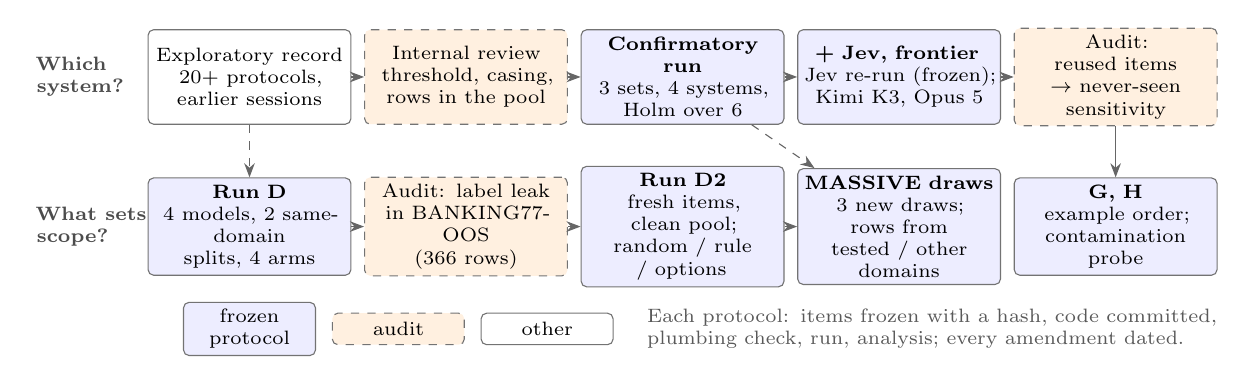
\begin{tikzpicture}[
  font=\scriptsize,
  every node/.style={align=center},
  box/.style={draw=black!55, rounded corners=2pt, inner sep=2.5pt, text width=24mm, minimum height=12mm},
  frozen/.style={box, fill=blue!7},
  audit/.style={box, fill=orange!12, dashed},
  plain/.style={box},
  lane/.style={font=\scriptsize\bfseries, text=black!70, text width=14mm, align=left},
  arr/.style={-{Stealth[length=1.8mm]}, draw=black!60}]

\def\dx{27.5mm}
% Lane labels
\node[lane] at (-20mm, 0) {Which\\system?};
\node[lane] at (-20mm, -19mm) {What sets\\scope?};

% Upper lane
\node[plain]  (expl)  at (0*\dx, 0) {Exploratory record\\20+ protocols,\\earlier sessions};
\node[audit]  (rev)   at (1*\dx, 0) {Internal review\\threshold, casing,\\rows in the pool};
\node[frozen] (conf)  at (2*\dx, 0) {\textbf{Confirmatory run}\\3 sets, 4 systems,\\Holm over 6};
\node[frozen] (front) at (3*\dx, 0) {\textbf{+ Jev, frontier}\\Jev re-run (frozen);\\Kimi K3, Opus 5};
\node[audit]  (fresh) at (4*\dx, 0) {Audit: reused items\\$\to$ never-seen\\sensitivity};

% Lower lane
\node[frozen] (rd)    at (0*\dx, -19mm) {\textbf{Run D}\\4 models, 2 same-\\domain splits, 4 arms};
\node[audit]  (leak)  at (1*\dx, -19mm) {Audit: label leak\\in BANKING77-OOS\\(366 rows)};
\node[frozen] (d2)    at (2*\dx, -19mm) {\textbf{Run D2}\\fresh items, clean pool;\\random / rule / options};
\node[frozen] (mr)    at (3*\dx, -19mm) {\textbf{MASSIVE draws}\\3 new draws; rows from\\tested / other domains};
\node[frozen] (gh)    at (4*\dx, -19mm) {\textbf{G, H}\\example order;\\contamination probe};

\foreach \a/\b in {expl/rev, rev/conf, conf/front, front/fresh, rd/leak, leak/d2, d2/mr}
  \draw[arr] (\a) -- (\b);
\draw[arr, dashed] (expl) -- (rd);
\draw[arr, dashed] (conf) -- (mr);
\draw[arr] (fresh) -- (gh);

% Key
\node[frozen, text width=15mm, minimum height=4mm] (k1) at (0*\dx, -32mm) {frozen protocol};
\node[audit, text width=15mm, minimum height=4mm, right=2mm of k1] (k2) {audit};
\node[plain, text width=15mm, minimum height=4mm, right=2mm of k2] (k3) {other};
\node[right=3mm of k3, text width=72mm, align=left, text=black!65] {Each protocol: items frozen with a hash, code committed, plumbing check, run, analysis; every amendment dated.};
\end{tikzpicture}
\caption{Study design. The upper lane compares systems that are given the same labelled data; the lower lane asks what sets a prompted model's out-of-scope decision. Dashed arrows mark where an observation in one study motivated another: the exploratory drop in same-domain rejection led to run D, and Gemma's 23\% rejection on MASSIVE led to the MASSIVE draws. Runs G and H check the confirmatory comparison. Filled boxes are protocols frozen before any of their requests; dashed boxes are audits recorded as dated errata.}
\label{fig:design}
\end{figure*}


\Cref{fig:design} shows how the experiments connect.

\paragraph{Decisions and endpoint.} Each turn needs a scope decision and, if in scope, an intent decision; a turn is right when both are. The primary endpoint is weighted turn accuracy, $0.8\times$ the share of in-scope turns kept with the right intent plus $0.2\times$ the share of out-of-scope turns rejected, which matches a 20\% out-of-scope prior and does not depend on the rate in the sessions. Turns form five-turn sessions; session success is secondary.

\paragraph{Data.} \Cref{tab:data} lists the confirmatory sets, built from Banking77 \citep{casanueva2020banking77}, MASSIVE \citep{fitzgerald2022massive} and CLINC150 \citep{larson2019clinc}. CLINC150 uses its native out-of-scope test queries, and Banking77 borrows the same CLINC150 queries. MASSIVE uses utterances from three whole domains held out of its label set (email, iot, play), drawn with a fixed seed from the 16 domains other than the catch-all \emph{general} and \emph{qa}, whose catch-all intents absorb out-of-scope requests \citep{li2024catchall}. Those are sibling domains of retained skills such as music and social. All text is lower-cased, and punctuation other than apostrophes is removed, for every system and pool. The sets were meant to contain only test items no earlier session used; that held for MASSIVE but not for Banking77 and CLINC150 (\cref{sec:freshness}).

\begin{table}[t]
\centering\small
\resizebox{\linewidth}{!}{%
\begin{tabular}{@{}lrrrr@{}}
\toprule
Set & Labels & Turns & Out of scope & Never seen \\
\midrule
Banking77 & 77 & 1,479 & 184 & 582 \\
MASSIVE & 42 & 1,216 & 243 & 1,215 \\
CLINC150 & 150 & 1,850 & 185 & 1,766 \\
\bottomrule
\end{tabular}}
\caption{Confirmatory sets. \emph{Never seen}: turns whose normalised text appears in no session built earlier (\cref{sec:freshness}). MASSIVE's in-scope turns cover 21 of its 42 labels.}
\label{tab:data}
\end{table}

\paragraph{Systems.}
\begin{itemize}
  \item \textbf{Specialist:} an Ettin 150M encoder \citep{weller2026ettin} with a mean-pooled classification head, retrained on the normalised data. It uses three seeds and a learning rate chosen on development data. Scope comes from a development-selected detector, with a threshold weighted by the 20\% prior.
  \item \textbf{General models:} Gemma 4 31B (primary) and Qwen3.5 27B (secondary). Each answers scope and intent at temperature 0 with reasoning off, after 20 BM25-nearest \citep{robertson2009bm25} in-scope training examples. The pool contains no out-of-scope rows, and labels are shown by name only, without descriptions.
  \item \textbf{Jev 1.13.0} \citep{deusser2026jev}: a hosted ``typed-decision'' model from TypeSafe, pinned to one version, that answers a yes/no question as a probability and a choice question as a distribution over the given labels in one call. Its weights and architecture are not public. It receives the same 20 neighbours, labelled with intent names, and its scope decision uses a fixed 0.5 threshold; its interface therefore differs from the general models' prompt, and comparisons with them are secondary.
  \item \textbf{Combination} (pre-registered): Gemma's scope, with the specialist's intent when its probability is at least 0.9.
  \item \textbf{Cascade} (pre-registered): the 40\% of turns with the lowest specialist confidence go to Gemma.
\end{itemize}
Hosts, precision, prompts and hyperparameters are in \cref{app:systems}.

\paragraph{Statistics.} Paired differences are tested by sign flips of cluster sums. Clusters are gold intents; each out-of-scope turn is its own cluster. Intervals are 95\% cluster bootstrap. The primary family is specialist against Gemma and combination against Gemma on each set, with Holm correction \citep{holm1979}. Banking77 was to be tested for equivalence at $\pm2.5$ points. Everything else is secondary and unadjusted, or post hoc where labelled.

% ---------------------------------------------------------------------------------------------------------------
\section{Confirmatory comparison}
\label{sec:confirmatory}

\begin{table*}[t]
\centering\small
\resizebox{\linewidth}{!}{%
\begin{tabular}{@{}lccccccccc@{}}
\toprule
& \multicolumn{6}{c}{Weighted turn accuracy (\%), all turns} & \multicolumn{2}{c}{Specialist $-$ Gemma (Holm $p$)} & \\
\cmidrule(lr){2-7}\cmidrule(lr){8-9}
Set & Specialist & Gemma & Qwen 27B & Combination & Cascade 0.4 & Jev + retr. & All turns & Never seen & Gemma \$/1k sess. \\
\midrule
Banking77 & 92.7 & 94.1 & 94.0 & 94.7 & 94.3 & 94.1 & $-1.42$ (.19) & $-1.65$ (.94) & 0.73 \\
MASSIVE & 78.3 & 73.8 & 80.8 & 74.4 & 73.5 & 77.8 & $+4.42$ (.51) & $+4.42$ (.94) & 0.47 \\
CLINC150 & 93.1 & 95.0 & 95.0 & 95.1 & 95.1 & 95.0 & $-1.89$ (\textbf{.007}) & $-0.94$ (.94) & 1.06 \\
\bottomrule
\end{tabular}}
\caption{Pre-registered comparison. Specialist: mean of three seeds. Combination and cascade use Gemma. Jev and Qwen are secondary. The \emph{never seen} column is a post hoc sensitivity analysis (\cref{sec:freshness}). The cascade calls Gemma on 40\% of turns, so it costs 40\% of the Gemma column; the combination calls it on every turn. Combination $-$ Gemma: $+0.58$, $+0.60$, $+0.10$ (Holm $\ge .40$).}
\label{tab:primary}
\end{table*}

\Cref{tab:primary} and \cref{fig:confirmatory} give the results. As pre-registered, the general model is ahead on CLINC150 by 1.9 points (Holm $p=.007$). On Banking77 the 1.4-point gap is not significant after correction. Equivalence within 2.5 points is indeterminate: the 90\% interval's lower bound is $-2.51$, with a standard deviation of 0.03 across bootstrap seeds. On MASSIVE the specialist is 4.4 points ahead, but the test cannot detect differences below about 9 points there, and Qwen is 2.6 points ahead of the specialist here and 1.9 to 3.4 points ahead on all three further draws (\cref{app:massive}), so the ranking depends on the model. The combination that looked better on our earlier data is level with Gemma on every set. The cascade is within 0.4 points of Gemma alone at 40\% of its API cost. Jev given the same retrieved examples is level with Gemma on Banking77 and CLINC150 (90\% intervals within $\pm0.9$ points) and 4.0 points ahead on the confirmatory MASSIVE draw ($p=.0001$, secondary), but not on the three further draws ($+0.5$, $-0.8$, $-3.5$). These gaps are not artefacts of example order: two further orderings of Gemma's 20 retrieved examples changed its weighted accuracy by at most 0.16 points on CLINC150 and 0.41 on MASSIVE, and left the CLINC150 gap between $-1.75$ and $-1.90$ (\cref{app:gh}).


\begin{figure*}[t]
\centering
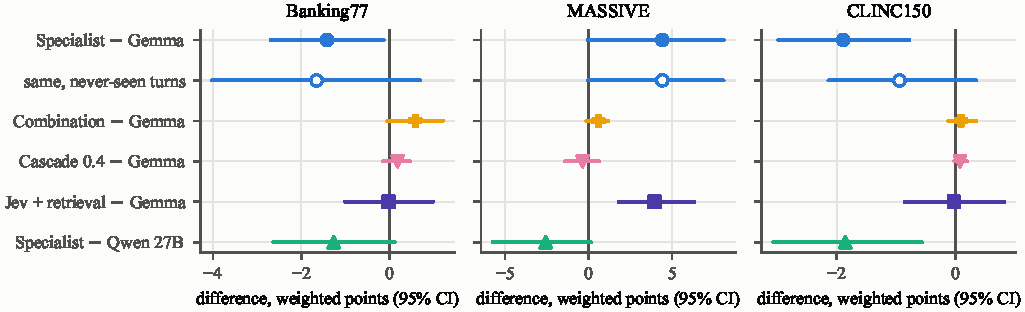
\includegraphics[width=\textwidth]{f6_confirmatory.pdf}
\caption{Paired differences in weighted turn accuracy with 95\% cluster-bootstrap intervals on the confirmatory sessions. Specialist $-$ Gemma is pre-registered; the never-seen row (open marker) is a post hoc sensitivity analysis; the other rows are pre-registered (combination, cascade) or secondary (Jev, Qwen). MASSIVE has almost no reused turns, so its two specialist rows coincide.}
\label{fig:confirmatory}
\end{figure*}

\paragraph{Where the gaps come from.} Splitting each gap into a scope part and an intent part, the CLINC150 gap divides evenly (0.9 scope, 1.0 intent). Our pre-registered headline rule therefore forbids saying that the difference lies in the out-of-scope decision. MASSIVE's 4.4 points are all scope. Gemma keeps 97\% of in-scope turns but rejects only 23\% of the held-out-domain requests: 5\% of \emph{play} requests, which it maps onto the retained music skills, and 35\% of \emph{email} requests. The specialist rejects 78\% and 81\% of these. Two frontier models answered the first 100 sessions of each set with the same prompt and reasoning off. Kimi K3 (2.8T parameters, open weights) and Claude Opus 5 also reject under 10\% of \emph{play} requests (\cref{app:frontier}). Without MASSIVE's catch-all \emph{general quirky} intent, which supplies 2.4 of the specialist's 7.1-point in-scope deficit, the specialist is 6.1 points ahead ($p=.001$, post hoc). On three further seeded draws of held-out domains (a sensitivity analysis that reuses MASSIVE test text; \cref{app:massive}), specialist minus Gemma is $-1.0$, $-1.7$ and $+0.3$ points, none significant, and Gemma rejects 61 to 68\% of held-out-domain requests. The further draws also held out music, the sibling of play, in two of three draws. The confirmatory MASSIVE result therefore depends on whether a sibling of a held-out domain remains among the skills. Clustering out-of-scope turns by their source label instead of by turn, the MASSIVE specialist $-$ Gemma difference has $p=.55$ (post hoc).

\paragraph{Freshness (post hoc).}
\label{sec:freshness}
After the run, an audit found that 832 of Banking77's 1,295 in-scope turns had been used before. So had 65 of its 184 out-of-scope turns and 78 of CLINC150's 185. They appeared in our exploratory BANKING77-OOS sessions. That set is a lower-cased copy of the Banking77 test split and reuses CLINC out-of-scope queries, and our freshness rule had matched exact text. The models never saw these items before, but we had. On never-seen turns no primary comparison is significant (\cref{tab:primary}); CLINC150's gap halves to $-0.94$ [$-2.14$, $+0.35$]. Split by component, the in-scope part of the CLINC150 gap is unchanged on never-seen turns ($-2.19$ [$-3.12$, $-1.32$], $p=.0001$). The change comes from the out-of-scope turns: specialist $-$ Gemma is $+4.0$ on the 107 never-seen ones and $-7.3$ on the 78 seen before. The reuse affected the out-of-scope comparison, not the in-scope one.

\paragraph{Frontier models and cost.} Kimi K3 and Claude Opus 5 are never significantly different from Gemma (largest: Opus on CLINC150, $+1.8$, $p=.065$), though 100 sessions per set cannot exclude gains of 2 to 3 points. Uncached at list prices they cost 17 to 21 and 36 to 44 times as much per session (\cref{app:frontier}). Hosting the specialist alone costs less than calling Gemma on every turn above about 47,000 to 106,000 sessions a month for a \$50-a-month host. The cascade still calls Gemma on 40\% of turns, so it pays for its hosting only above about 79,000 to 177,000 sessions a month. The specialist's median latency is 11\,ms on one consumer GPU; median call latency is 1.0\,s for Gemma, 2.3\,s for Qwen, 2.8\,s for Kimi K3 and 1.2\,s for Claude Opus 5 (\cref{app:systems}).

% ---------------------------------------------------------------------------------------------------------------
\section{What sets a prompted model's out-of-scope decision}
\label{sec:operating}

\begin{table*}[t]
\centering\small
\resizebox{\linewidth}{!}{%
\begin{tabular}{@{}lcccccc@{}}
\toprule
& \multicolumn{3}{c}{BANKING77-OOS: held-out rejected (\%)} & In-scope kept (\%) & \multicolumn{2}{c}{CLINC single-domain} \\
\cmidrule(lr){2-4}\cmidrule(lr){6-7}
Model & As run & Leak-free subset & Instruction (as run) & zero-shot $\to$ retrieval & Held-out rejected & Instruction \\
\midrule
Gemma 4 31B & 59.5 $\to$ 30.3 & 67.5 $\to$ 42.9 & 33.3 & 91.7 $\to$ 98.2 & 42.6 $\to$ 47.6 & 70.3 \\
Qwen3.5 27B & 82.2 $\to$ 58.5 & 85.4 $\to$ 71.2 & 63.5 & 80.9 $\to$ 95.2 & 67.0 $\to$ 68.9 & 84.1 \\
Llama 3.3 70B & 50.7 $\to$ 17.7 & 69.2 $\to$ 31.7 & 31.7 & 89.2 $\to$ 99.2 & 34.4 $\to$ 39.4 & 66.6 \\
DeepSeek V4 Pro & 60.8 $\to$ 21.1 & 70.4 $\to$ 38.3 & 31.8 & 88.9 $\to$ 99.0 & 30.6 $\to$ 31.7 & 48.6 \\
Jev 1.13.0 & 70.7 $\to$ 25.3 & 79.2 $\to$ 50.4 & 25.5 & 88.7 $\to$ 98.2 & 55.4 $\to$ 56.9 & 61.7 \\
\midrule
Specialist (reference) & \multicolumn{2}{c}{49.6 (44.5 on dev-unseen intents)} & & & 53.7 (37.9 dev-unseen) & \\
\bottomrule
\end{tabular}}
\caption{Rejection of held-out same-domain requests, zero-shot $\to$ retrieval of 20 in-scope examples. The drop on BANKING77-OOS is pre-registered for each model (Holm $p\le.0008$). On the post hoc leak-free subset (10 held-out intents that never leak, label-clean items) it is 14 to 38 points, $p\le.009$ each. On CLINC single-domain, retrieval leaves rejection level or raises it by 1 to 5 points, and no model shows a drop. \emph{Instruction}: the retrieval prompt plus one sentence on scope.}
\label{tab:suppression}
\end{table*}

On our exploratory BANKING77-OOS sessions, Gemma rejected 70\% of requests for held-out Banking77 intents zero-shot and 38\% with retrieved in-scope examples. A second frozen protocol tested this on fresh items, with four general models from four families and two same-domain splits: BANKING77-OOS \citep{zhang2022oos}, and CLINC single-domain out-of-scope for banking and for credit cards. There were four arms: zero-shot, retrieval, retrieval with a scope instruction, and retrieval with four fixed off-topic out-of-scope examples. The Jev protocol repeated the first three arms.

\paragraph{Retrieval moves models towards acceptance on one split.} On BANKING77-OOS, retrieval lowered rejection of held-out requests for all four general models, by 24 to 40 points (Holm $p=.0008$ each), and for Jev by 45 points (Holm $p=.0002$; \cref{tab:suppression}). It also raised in-scope acceptance from 81--92\% to 95--99\%. On CLINC single-domain it lowered rejection for no model.

An audit then found that the published BANKING77-OOS training split mislabels 366 of 5,905 rows. 145 of them are utterances of 17 held-out intents filed under in-scope labels, so the retrieval pool leaked held-out intents, and the models copied the leaked labels. On the 10 held-out intents that never leak, the drop is 14 to 38 points for all five models ($p\le.009$). It survives the leak but is smaller.

\paragraph{Mechanism (post hoc for the general models, pre-registered for Jev).} Accepted held-out requests go to nearby in-scope labels whose examples were retrieved (D2 items below; \cref{app:posthoc}). For the four general models, the chosen label is among the 20 retrieved labels for 92 to 99\% of accepted held-out requests. Gemma, for example, maps all 33 identity-verification requests it accepts to \emph{why verify identity}. The drop is larger where the retrieved labels concentrate on one label (for Qwen, 29 points against 8). As an aggregate description we treat scope as a detection task \citep{macmillan2005detection}, separating discrimination ($d'$) from the criterion ($c$, readiness to accept). On leak-free BANKING77-OOS items, retrieval moves the four general models' criterion towards acceptance by 0.7 to 1.1 standard deviations. Allowing unequal variances (zROC slopes 0.6 to 1.25), discrimination improves for Llama and DeepSeek at every slope, while for Gemma and Qwen the sign of the change depends on the slope.

Jev returns probabilities, so its discrimination was measured directly. Its pre-registered readout on the as-run items was an operating-point shift: AUROC unchanged ($+0.003$ [$-0.03$, $+0.04$]), and the mean in-scope probability on held-out requests up by 0.29. On leak-free items its AUROC rises slightly ($+0.03$ [$+0.007$, $+0.068$]) while that mean probability still rises by 0.17. The consistent reading is that retrieved examples of sibling labels draw unsupported requests into those labels, which in aggregate looks like a shift towards acceptance with level or slightly better discrimination.

On CLINC single-domain the shift is smaller (the interval excludes zero for two of four general models), and discrimination improves (Jev: AUROC $+0.11$). Retrieval closeness does not explain the difference between the splits once the leak is removed (AUROC of top-1 similarity 0.90 against 0.91).


\begin{figure*}[t]
\centering
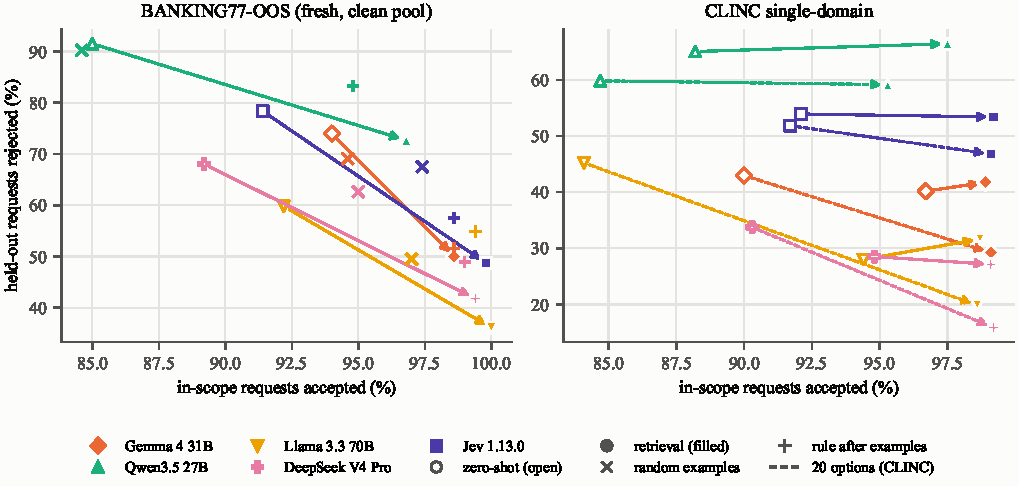
\includegraphics[width=\textwidth]{f7_operating_points.pdf}
\caption{Operating points of the scope decision in run D2. Each arrow runs from a model's zero-shot answer (open marker) to its answer with 20 retrieved in-scope examples (filled marker). On BANKING77-OOS every model moves down and to the right: it accepts more in-scope requests and rejects fewer unsupported ones. Random examples ($\times$) move it much less, and repeating the scope rule after the examples ($+$) moves it back for four of five models. On CLINC single-domain the 10-option prompts (solid) barely move the rejection rate, while the 20-option prompts (dashed) move three models down.}
\label{fig:operating}
\end{figure*}

\paragraph{Replication and causes (pre-registered, run D2).} A third frozen protocol used fresh, label-clean validation items. On BANKING77-OOS there were 500 in-scope and 388 held-out items, from 23 intents, with all 366 mislabelled rows removed from the pool. On CLINC single-domain there were 1,000 in-scope and 575 held-out items. The protocol added three arms (\cref{tab:d2,fig:operating}).
\begin{itemize}
  \item \textbf{The drop replicates} for all five models, by 19 to 30 points (Holm $p\le.0006$).
  \item \textbf{Relevance drives it.} Twenty random in-scope examples leave rejection 13 to 21 points higher than the 20 retrieved ones (Holm $p\le.004$ for all five), within 1 to 11 points of zero-shot.
  \item \textbf{Repeating the rule partly helps.} Repeating the scope rule after the examples, immediately before the request, recovers 7 to 19 points of rejection for Qwen, Llama, DeepSeek and Jev (Holm $p\le.008$); Gemma does not move ($+1.5$, $p=.13$). By run D's ``works'' criterion this is a mitigation for Llama only (79\% recovered at $-0.6$ in-scope points). The arm repeats the rule rather than moving it.
  \item \textbf{Option count is not established.} With CLINC single-domain's two domains pooled into one 20-option prompt, retrieval lowers rejection for four of five models, most for Gemma (43 to 29\%), Llama (45 to 20\%) and DeepSeek (34 to 16\%). The difference from the 10-option prompts is Holm-significant only for Llama ($-29$ points, $p=.04$), but with eight held-out-intent clusters and Holm over five models, $.04$ is the smallest attainable adjusted $p$. The pooled prompt also adds sibling labels from the other domain, mixes the retrieval pools and changes the desk description, and its effect differs in sign between the two domains, so this arm does not isolate option count.
\end{itemize}
Throughout, the aggregate criterion moves towards acceptance; Jev's AUROC rises from 0.934 to 0.965, so for it discrimination does not fall.

\begin{table}[t]
\centering\small
\resizebox{\linewidth}{!}{%
\begin{tabular}{@{}lcccc@{}}
\toprule
Model & Zero-shot & Retrieval & Random & Rule after \\
\midrule
Gemma 4 31B & 74.0 & 50.0 & 69.1 & 51.5 \\
Qwen3.5 27B & 91.5 & 72.7 & 90.2 & 83.2 \\
Llama 3.3 70B & 59.8 & 36.1 & 49.5 & 54.9 \\
DeepSeek V4 Pro & 68.0 & 41.8 & 62.6 & 49.0 \\
Jev 1.13.0 & 78.4 & 48.7 & 67.5 & 57.5 \\
\bottomrule
\end{tabular}}
\caption{Run D2: held-out rejection (\%) on fresh label-clean BANKING77-OOS items with a clean pool. \emph{Random}: 20 random in-scope examples. \emph{Rule after}: the scope rule repeated after the retrieved examples. In-scope acceptance is 85--94\% zero-shot and 97--100\% with retrieval.}
\label{tab:d2}
\end{table}


\begin{figure}[t]
\centering
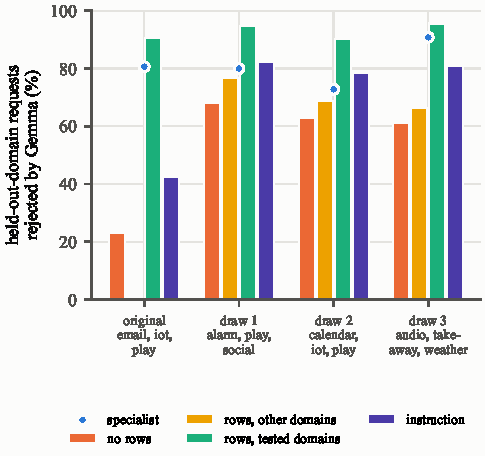
\includegraphics[width=\linewidth]{f8_massive_rows.pdf}
\caption{Gemma's rejection of held-out-domain MASSIVE requests on the confirmatory draw and three further draws (sensitivity analysis), with the specialist for reference. Labelled out-of-scope rows from the tested domains raise rejection most; rows from other unsupported domains raise it less, and only for requests that retrieve them.}
\label{fig:rows}
\end{figure}

\paragraph{Labelled unsupported examples move it the other way.} In a paired secondary arm of the confirmatory run, we added 250 labelled out-of-scope rows to Gemma's pool. These rows came from the same three held-out domains as the test requests. Gemma's rejection of those requests rose from 23\% to 91\%, and its weighted accuracy rose by 13.3 points [12.1, 14.6]. With the same rows offered to the specialist, its development-selected rule used them only on MASSIVE, and there the two were level ($-1.8$, $p=.54$). On the three further MASSIVE draws, rows from the tested domains again raised accuracy, for Gemma by 5.1 to 6.5 points and for Qwen by 2.3 to 4.0 (Holm $p=.0003$ for all six). Rows from three \emph{other} unsupported domains raised weighted accuracy significantly in 1 of 6 tests (Gemma, draw 1, $+2.0$), but raised rejection in all 6 cells (post hoc, $+2.4$ to $+8.8$ points). That gain falls on the requests for which such a row is retrieved ($+5$ to $+16$ points, against about zero for the others). A one-sentence scope instruction did not help significantly ($+1$ to $+2$ points for Gemma). Labelled out-of-scope examples help a prompted model on the requests that retrieve them (\cref{fig:rows}). Clustering run C's out-of-scope turns by their source label, its rows effect has $p=.03$ (post hoc).

\paragraph{Mitigations.} Neither pre-registered mitigation met its criterion, which was to recover half of the lost rejection at a cost of at most 2 points of in-scope accuracy. The instruction recovered 10 to 42\% on BANKING77-OOS and none for Jev. On CLINC single-domain it raised rejection by 15 to 27 points for the general models, and by 5 points for Jev. On either split it cost at most 1.8 in-scope points. Off-topic out-of-scope examples did not help. In D2, repeating the scope rule after the examples met the criterion for Llama only. Two post hoc rules on the saved answers also fail the criterion on held-out intents that the development items did not cover (\cref{app:posthoc}). Accepting only when the specialist also accepts recovers 42 to 96\% of the loss at 2.0 to 3.0 in-scope points. A similarity floor costs 11 to 16 points.

% ---------------------------------------------------------------------------------------------------------------
\section{Discussion}

The answer to our opening question is that the kind of model matters less than what it is given. With the same labelled examples, a 150M classifier, 27--31B prompted models, two frontier models and a typed-decision model land within a few points of each other. The typed-decision model, the newest of these, behaves like the prompted models, including the drop in its rejection of unsupported requests when in-scope examples are retrieved. For a team choosing a system, the deciding factors are therefore practical: whether labelled data exists, what each call costs, and how out-of-scope requests are sourced and shown to the model. Four observations follow, each tagged with its evidence:
\begin{enumerate}
  \item \textbf{Matched and equipped, the systems are close} (pre-registered). They differ by less than two points on Banking77 and CLINC150, and MASSIVE's direction depends on the model. A 31B general model, a typed-decision model and a 150M classifier given the same examples are within a few points of each other, and much larger models add little. Claims that one approach dominates should be checked against an equipped version of the other.
  \item \textbf{For a prompted model, the out-of-scope decision moves with what the prompt shows.} Retrieved in-scope examples lower the rejection of unsupported same-domain requests on BANKING77-OOS (pre-registered twice, the second time on fresh leak-free items for five models). Relevant, not random, examples cause it, and the accepted requests go to sibling labels whose examples were retrieved (post hoc). They did not lower rejection on CLINC single-domain with 10 options, and we could not establish why. Labelled out-of-scope examples raise rejection for the requests that retrieve them (MASSIVE, four draws). Repeating the scope rule after the examples helped four of five models but met our mitigation criterion for one. The classifier's threshold, by contrast, is tuned on development data. A fair comparison reports each system's operating point, not only its accuracy.
  \item \textbf{Comparisons of this kind are fragile.} Our exploratory MASSIVE result (Gemma $+5.3$) did not survive the confirmatory design, which changed the label set, the out-of-scope source, the casing and the pool at once. A public benchmark leaked held-out intents into its training split. Our own freshness rule missed lower-cased copies. We suggest reporting, for any classifier-versus-model scope comparison: how out-of-scope data was sourced and whether surface cues separate it, what data each system's scope decision could use, the objective behind every threshold, and a label audit of the benchmark.
  \item \textbf{The cascade's value is API cost} (pre-registered). It comes within 0.4 points of the general model at 40\% of its API cost, but it also needs the classifier hosted, which pays for itself only above about 79,000 to 177,000 sessions a month at \$50 a month.
\end{enumerate}

\section*{Limitations}

\paragraph{Data.}
\begin{itemize}
  \item The confirmatory sets are assembled from single utterances of three English label sets.
  \item The supply of native out-of-scope data limits their size: the smallest detectable differences are 1.7, 1.9 and 8.8 points.
  \item Banking77 and CLINC150 items overlap our exploratory sessions.
  \item The confirmatory MASSIVE draw held out sibling domains, and three further draws reuse its test text. Its in-scope turns cover half of its labels.
  \item Run C's rows come from the test domains.
  \item The two same-domain splits come from one benchmark family. One of them has a label leak, and they differ in option count.
  \item The base BANKING77-OOS prompt already contains a scope sentence.
  \item Labels are shown by name only; label descriptions might reduce sibling absorption.
  \item The option-count arm could reach significance for at most one model and changes more than the number of options.
  \item The further MASSIVE draws hold out six domains each, which removes sibling skills from the label set.
\end{itemize}

\paragraph{Models.}
\begin{itemize}
  \item General models ran once per prompt at temperature 0 with one retriever; other orders of the retrieved examples changed accuracy by at most 0.4 points.
  \item Moving one model between two fp8 hosts changed 9.5\% of its answers, which is the size of several reported differences.
  \item Frontier models were limited to those accepting reasoning disabled.
  \item Jev's per-call price is not reported by its API; all Jev use in the project, including exploratory calls before the frozen runs, cost \$4.27 from a prepaid balance, so a per-call price cannot be separated. Its interface (a fixed probability threshold, label names) differs from the general models' prompt.
\end{itemize}

\paragraph{Analyses.}
\begin{itemize}
  \item The specialist uses development out-of-scope data; the prompted models use none.
  \item The signal-detection estimates for the general models are aggregate descriptions; under unequal variances the sign of the discrimination change is not determined for two of four models.
  \item CLINC150 and Banking77 are public and may be in the models' training data. A completion probe found 0.5\% verbatim completions for Gemma (Qwen refused the task), which does not rule contamination out.
\end{itemize}

\section*{Availability and licences}
Protocols, frozen item lists, every saved model reply, analysis code and the record of withdrawn conclusions are in our release (\texttt{release/README.md}, with SHA-256 hashes of every file); specialist weights and features are archived separately against the same hashes. % OWNER: add the public link before submission.
Banking77 is CC BY 4.0, CLINC150 CC BY 3.0 and MASSIVE CC BY 4.0. BANKING77-OOS and CLINC single-domain out-of-scope \citep{zhang2022oos} state no licence; we do not redistribute them.

\section*{Disclosures}
\textbf{Jev.} The author has no affiliation with TypeSafe, the provider of Jev, and received no funding or special access from it. Jev was used through its API in the same way as the other hosted models.

\textbf{AI assistance.} The author conceived and designed the study, chose the data sets, models and hypotheses, approved every protocol before it ran, directed the analyses and the internal review rounds, and is responsible for all content. AI tools assisted with coding and editing.

\bibliography{references}

\appendix

\section{Protocols, amendments and withdrawn conclusions}
\label{app:record}

The confirmatory questions were chosen after more than twenty exploratory protocols on the same label sets. Six protocols govern this paper; each was committed before any of its requests, and each carries dated amendments:
\begin{itemize}
  \item \texttt{confirmatory\_protocol.json}
  \item \texttt{retrieval\_suppression\_protocol.json}
  \item \texttt{jev\_rerun\_protocol.json}
  \item \texttt{retrieval\_mechanism\_protocol.json}
  \item \texttt{massive\_robustness\_protocol.json}
  \item \texttt{gh\_protocol.json}
\end{itemize}
The amendments are:
\begin{itemize}
  \item the frontier model was changed after Qwen3.8 2.4T refused requests with reasoning disabled;
  \item a plumbing-check cap was raised;
  \item DeepSeek V4 Pro was moved between hosts after rate limits;
  \item errata record the freshness problem (\cref{sec:freshness}) and the BANKING77-OOS label leak;
  \item run D's BANKING77-OOS items were fresh with respect to the BANKING77-OOS sessions only: 462 of its 1,077 items had appeared as confirmatory Banking77 turns;
  \item before freezing D2, its CLINC single-domain in-scope items were allowed although they had served as run D's specialist development data (never sent to a model);
  \item D2 was switched to one process per model about an hour after its requests began (a request-loop change only; its note miscounts the finished cells), and the per-process caps together exceeded the run cap, which spend never approached;
  \item the cost figure stage of \texttt{confirmatory.py} was edited after the run (presentation only).
\end{itemize}
Two parallel processes briefly sent 76 duplicate requests, and spend was reconciled from saved rows. Every request of every experiment was answered; parse failures were zero in all runs.

Conclusions of our earlier drafts that these runs withdrew or narrowed:
\begin{enumerate}
  \item that the retrieval-prompted model overtakes the classifier on Banking77, MASSIVE and CLINC150;
  \item that the combination of the model's scope and the classifier's intent is significantly better on Banking77;
  \item that the difference lies in the out-of-scope decision;
  \item that BANKING77-OOS held-out requests resemble the retrieval pool more closely than CLINC single-domain ones (an artefact of the leak);
  \item that Jev is a weak scope gate. That came from zero-shot runs on our exploratory sessions; with retrieval it is level with Gemma on two sets;
  \item that the systems differ mainly in where they put the out-of-scope threshold (draft 3 abstract; contradicted by the pre-registered headline rule);
  \item that restating the scope rule after the examples is a cheap general lever (it met the mitigation criterion for one of five models);
  \item that labelled out-of-scope rows help only when they come from the tested domains (rows from other domains raise rejection for the requests that retrieve them);
  \item that Gemma's host was slow throughout runs G and H (the saved latencies give medians of about one second).
\end{enumerate}
Studies cut from this paper remain in the release record: typed state against stated decisions, model-to-model handoff, encoder against decoder, a local orchestrator, de-escalation and cascades between two general models.

\section{Systems and prompts}
\label{app:systems}

\begin{table*}[t]
\centering\small
\resizebox{\linewidth}{!}{%
\begin{tabular}{@{}llll@{}}
\toprule
Model & Host & Precision & Price, \$ per million input / output \\
\midrule
Gemma 4 31B & Novita & bf16 & 0.14 / 0.40 \\
Qwen3.5 27B & Alibaba & not stated & 0.195 / 1.56 \\
Llama 3.3 70B & DeepInfra & fp8 & 0.10 / 0.32 \\
DeepSeek V4 Pro & StreamLake & fp8 & 0.955 / 1.911 \\
Kimi K3 & Moonshot AI & mxfp4 & 3 / 15 \\
Claude Opus 5 & Anthropic & not stated & 5 / 25 \\
Jev 1.13.0 & TypeSafe & not stated & not reported per call \\
\bottomrule
\end{tabular}}
\end{table*}

\paragraph{Settings.}
\begin{itemize}
  \item \textbf{Prices and hosts:} prices are OpenRouter listings for the pinned host, 15--16 October 2026, with fallbacks off.
  \item \textbf{Retrieval:} BM25 with $k_1=1.5$ and $b=0.75$ over lower-cased word tokens, top 20, listed least similar first as ``message $\Rightarrow$ code''.
  \item \textbf{Specialist training:} learning rate and epochs chosen on development data from $\{2\cdot10^{-5},5\cdot10^{-5},10^{-4},2\cdot10^{-4}\}\times\{3,6\}$, with seeds 20261007, 20261015 and 20261016.
  \item \textbf{Specialist scope detectors:} softmax, energy, Mahalanobis and tenth-nearest neighbour.
  \item \textbf{Specialist development data:} 400 in-scope and 100 out-of-scope items.
  \item \textbf{Prompts:} reproduced verbatim in the protocol files, together with the session sampler and its seeds.
  \item \textbf{Latency per call} on the confirmatory runs (p50 / p95 / p99, seconds): Gemma 1.0 / 8.8 / 40.0 (including a host slowdown), Qwen 2.3 / 10.7 / 13.3, Kimi K3 2.8 / 5.3 / 7.7, Claude Opus 5 1.2 / 2.0 / 4.2; the specialist 0.011 / 0.013 on one RTX 5070. Jev's latency was not recorded.
\end{itemize}

\section{Frontier models and cost}
\label{app:frontier}

\begin{table*}[t]
\centering\small
\resizebox{\linewidth}{!}{%
\begin{tabular}{@{}lccccc@{}}
\toprule
Set (first 100 sessions) & Specialist & Gemma 4 31B & Kimi K3 & Claude Opus 5 & Uncached cost, multiple of Gemma (Kimi / Opus) \\
\midrule
Banking77 & 93.0 & 95.0 & 95.9 & 95.9 & 20.5 / 44.1 \\
MASSIVE & 80.4 & 78.5 & 79.0 & 77.2 & 21.3 / 43.0 \\
CLINC150 & 93.2 & 95.9 & 95.1 & 97.6 & 17.4 / 36.1 \\
\bottomrule
\end{tabular}}
\end{table*}

\begin{figure*}[t]
\centering
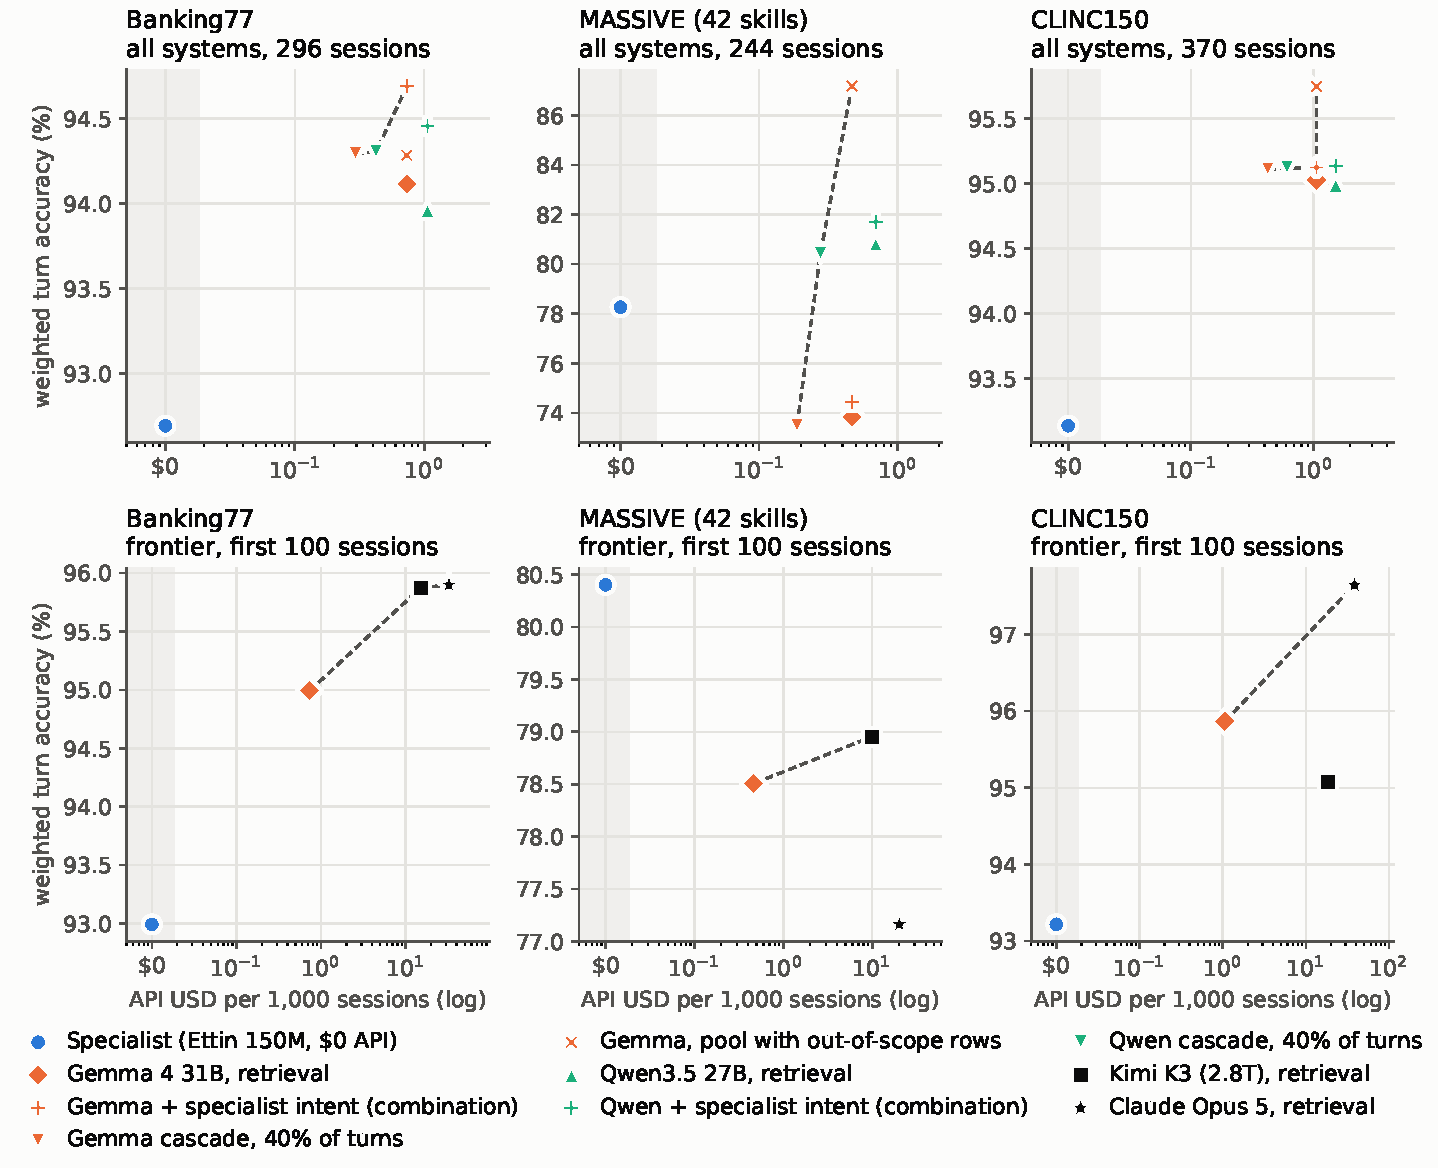
\includegraphics[width=\textwidth]{f5_cost_frontier.pdf}
\caption{Weighted turn accuracy against API cost per 1,000 sessions at uncached list prices; the dashed line is the frontier of systems with an API cost. The specialist has no API cost and is drawn in the shaded off-scale band; its hosting cost is not shown. Jev is not shown because its API does not report a per-call price.}
\end{figure*}

\section{Post hoc analyses}
\label{app:posthoc}

\paragraph{Mitigation rules.} The full tables are in \texttt{docs/posthoc-round3.md} and \texttt{docs/posthoc-round3b.md}. The development out-of-scope items covered 5 of the 27 held-out test intents on BANKING77-OOS, and 2 of 5 per CLINC single-domain domain. The specialist rejects 64.8\% of covered-intent requests against 44.5\% of uncovered ones. On uncovered intents only:
\begin{itemize}
  \item \textbf{Classifier veto} (accept only if the specialist also accepts): recovers 42 to 96\% of the lost rejection on BANKING77-OOS, at 2.0 to 3.0 points of in-scope accuracy, with every interval extending below $-2$.
  \item \textbf{Similarity floor:} costs 11 to 16 points.
  \item \textbf{Neighbour-label rule:} changes little.
\end{itemize}

\paragraph{Sibling labels (D2, BANKING77-OOS, retrieval).} Gemma's accepted held-out requests go mostly to sibling labels: verify my identity and unable to verify identity to \emph{why verify identity} (17 and 16), pin blocked to \emph{change pin} (15), top-up by bank transfer charge to \emph{transfer fee charged} (10). The chosen label is among the 20 retrieved labels for 92 to 99\% of accepted held-out requests and is the top-1 neighbour's label for 43 to 58\% (four general models). Split at the median concentration of the retrieved labels, rejection falls by 30 against 18 points (Gemma), 29 against 8 (Qwen), 25 against 23 (Llama) and 30 against 22 (DeepSeek).

\paragraph{Label audit.} BANKING77-OOS was matched to the original Banking77 labels after lower-casing:
\begin{itemize}
  \item 366 mislabelled training rows, of which 145 are leaked held-out intents;
  \item 32 in-scope test items with wrong gold intents;
  \item 36 ``held-out'' test items that are in-scope intents by their original labels.
\end{itemize}
Our files are byte-identical to the upstream release.

\section{MASSIVE robustness (sensitivity analysis)}
\label{app:massive}

A frozen protocol (\texttt{massive\_robustness\_protocol.json}) drew three further sets of three held-out test domains: alarm, play and social; calendar, iot and play; audio, takeaway and weather. Each draw also held out three domains that supplied labelled out-of-scope rows. Each draw has 1,000 in-scope and 250 out-of-scope test utterances, and the specialist was retrained per draw.

\begin{table*}[t]
\centering\small
\resizebox{\linewidth}{!}{%
\begin{tabular}{@{}lcccc@{}}
\toprule
Weighted accuracy / held-out rejected (\%) & Draw 1 & Draw 2 & Draw 3 & Original \\
\midrule
Specialist & 83.1 / 80.0 & 83.1 / 72.8 & 82.3 / 90.8 & 78.3 / 80.7 \\
Gemma, no rows & 84.1 / 68.0 & 84.7 / 62.8 & 82.0 / 61.2 & 73.8 / 23.0 \\
Gemma, rows from the tested domains & 89.7 / 94.8 & 89.8 / 90.4 & 88.5 / 95.6 & 87.2 / 90.5 \\
Gemma, rows from other domains & 86.1 / 76.8 & 85.5 / 68.8 & 82.3 / 66.4 & -- \\
Gemma, instruction & 85.5 / 82.4 & 85.8 / 78.4 & 84.0 / 80.8 & 75.3 / 42.4 \\
Qwen 27B, no rows & 86.5 / 82.8 & 85.3 / 72.8 & 84.2 / 81.6 & 80.8 / 68.3 \\
Jev, no rows & 84.6 / 70.4 & 83.9 / 56.4 & 78.5 / 47.6 & 77.8 / 44.0 \\
\bottomrule
\end{tabular}}
\end{table*}

\section{Example order and contamination (runs G and H)}
\label{app:gh}

A frozen protocol (\texttt{gh\_protocol.json}) re-ran Gemma on the confirmatory CLINC150 and MASSIVE turns with the 20 retrieved examples most similar first and in a random order, in addition to the original least-similar-first order. Weighted accuracy ranged over 0.16 points on CLINC150 and 0.41 on MASSIVE; 0.6 to 4.5\% of answers changed. A contamination probe asked Gemma and Qwen to complete the second half of 200 Banking77 and 200 CLINC150 test utterances. Gemma completed 0.5\% verbatim. Its completions resembled their own endings more than other endings of the same intent (token F1 0.18 against 0.08 on Banking77); this probe cannot tell that apart from memorisation. Qwen refused 350 of 400 requests, so its rows say little. The pre-registered criterion for memorisation (a significant own-ending advantage and more than 5\% verbatim) was not met.

\section{Exploratory record}
\label{app:exploratory}

On our earlier sessions, a model retrieving from exactly the rows the specialist was trained on was never significantly behind it at any training-set size. This used one seed, one model, and a pool with out-of-scope rows. At one example per intent no specialist was usable, while nearest-neighbour and centroid classifiers on the same rows got 14\% of Banking77 sessions against about 49\% for the retrieval-prompted model.

On MultiDoGO support chats, the specialist was more accurate on the dataset's ``out of domain'' label and, by under one point, on its dialogue-act labels. Gemma was more accurate on task intents; Qwen 27B's difference there was not significant.

\end{document}
